\subsubsection{Interrupt Funktionen (NVIC)}
\label{sec:CubeMXNVIC}

Neben den Systeminterrupts sind folgende Hardwareinterrupts aktiviert.
Für die Abarbeitung des I\textsuperscript{2}S2 DMA Datastreams sind die Interrupts \texttt{DMA1 Stream3} (Peripheral To Memory) sowie \texttt{DMA1 Stream4} )(Memory To Peripheral) aktiviert.
Zudem sind folgende GPIO Interrupts (EXTI) für die Buttons und Encoder Buttons aktiviert.

\begin{table}[H]
	\centering
	\begin{tabular}{|l|l|l|}
		\hline
		\textbf{Port} & \textbf{EXTI} & \textbf{Signal}  \\ \hline
		PA0           & EXTI0         & User Button SW1  \\ \hline
		PA1           & EXTI1         & User Button SW2  \\ \hline
		PC12          & EXTI12        & Encoder 1 Button \\ \hline
		PB13          & EXTI13        & Encoder 2 Button \\ \hline
	\end{tabular}
\end{table}

\begin{figure}[H]
	\centering
	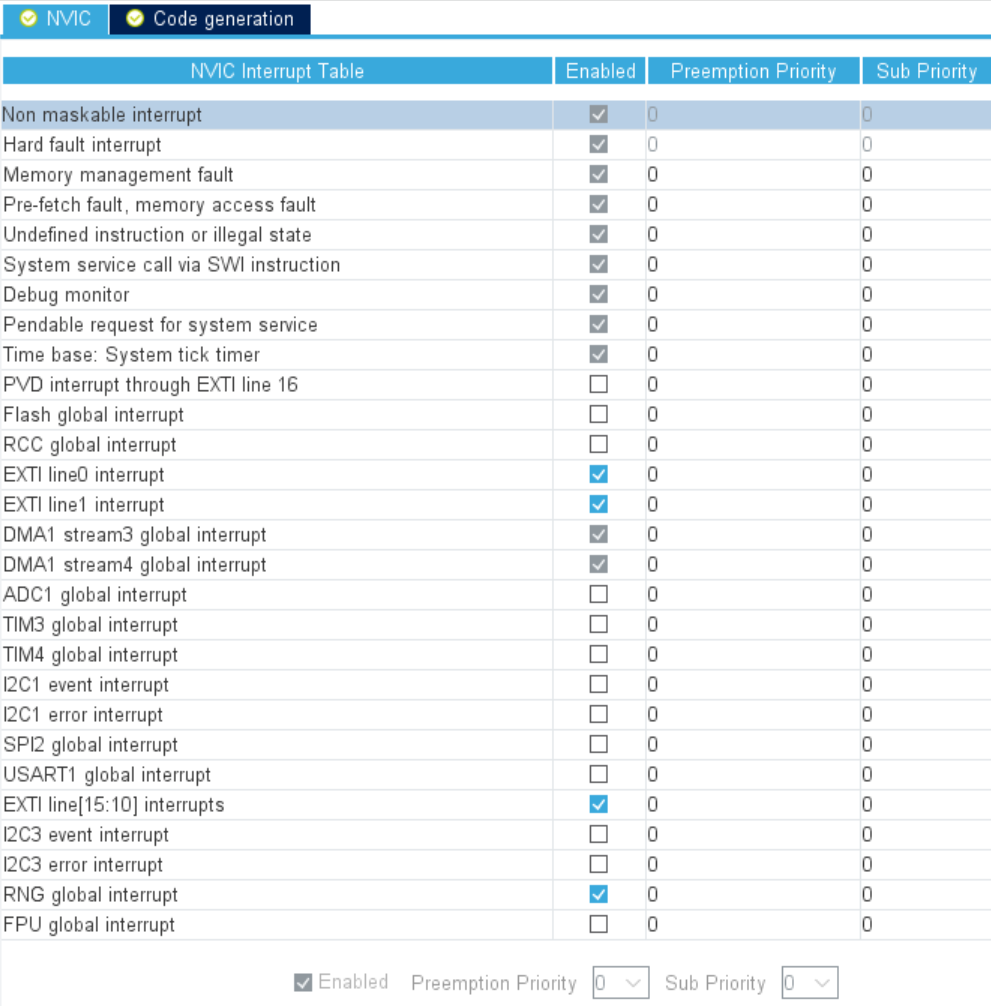
\includegraphics[width=0.9\linewidth]{CubeMX_NVIC}
	\caption{Alle aktivierten Interrupts }
	\label{pic:CubeMX_NVIC}
\end{figure}


